\documentclass{beamer}
\usetheme[white]{Wisconsin}
\usepackage{wrapfig}
\usepackage{longtable}
\usepackage{listings}
\usepackage{color}
%% The amssymb package provides various useful mathematical symbols
\usepackage{amssymb}
%% The amsthm package provides extended theorem environments
\usepackage{amsthm} \usepackage{amsmath}
\usepackage[mathcal]{euscript} \usepackage{color}
\usepackage{textcomp}
\usepackage{algorithm,algorithmic}
\usepackage[absolute,overlay]{textpos}
  \setlength{\TPHorizModule}{1mm}
  \setlength{\TPVertModule}{1mm}
\definecolor{listinggray}{gray}{0.9}
\definecolor{lbcolor}{rgb}{0.9,0.9,0.9}
\lstset{
  backgroundcolor=\color{lbcolor},
  tabsize=4,
  rulecolor=,
  language=c++,
  basicstyle=\scriptsize,
  upquote=true,
  aboveskip={1.5\baselineskip},
  columns=fixed,
  showstringspaces=false,
  extendedchars=true,
  breaklines=true,
  prebreak =
  \raisebox{0ex}[0ex][0ex]{\ensuremath{\hookleftarrow}},
  frame=single,
  showtabs=false,
  showspaces=false,
  showstringspaces=false,
  identifierstyle=\ttfamily,
  keywordstyle=\color[rgb]{0,0,1},
  commentstyle=\color[rgb]{0.133,0.545,0.133},
  stringstyle=\color[rgb]{0.627,0.126,0.941},
}

%% colors
\setbeamercolor{boxheadcolor}{fg=white,bg=UWRed}
\setbeamercolor{boxbodycolor}{fg=black,bg=white}

\setbeamerfont{block body}{size=\footnotesize}

%%----------------------------------------------------------------------------%%
\author{Alex P. Robinson
    \\ Engineering Physics Department
    \\ University of Wisconsin - Madison
    \\ Preliminary Examination
}

\date{\today}
\title{Development of a Monte Carlo Code System with Continuous Energy Adjoint Transport Capabilities for Neutrons and Photons} 
\begin{document}
\maketitle
%%----------------------------------------------------------------------------%%
\section{Overview}
%%----------------------------------------------------------------------------%%
\begin{frame}{Overview}

\begin{itemize}
  \item The Monte Carlo method
  \item Motivations for using the adjoint process
  \item Monte Carlo codes available today
  \item The Monte Carlo random walk process
  \item The Monte Carlo random walk process for radiation transport
  \item The Monte Carlo random walk process for adjoint radiation transport
  \item Adjoint photon incoherent scattering
  \item Adjoint photon coherent scattering
  \item Adjoint photon pair production
  \item The adjoint photon weight factor
  \item FACEMC code overview
  \item FACEMC validation plan
  \item Future Work
\end{itemize}

\end{frame}

%%----------------------------------------------------------------------------%%
\section{The Monte Carlo Method}
%%----------------------------------------------------------------------------%%
\begin{frame}{The Monte Carlo method}

  \begin{itemize}
    \item The Monte Carlo method is a stochastic method in which samples are
      drawn from a parent population through sampling procedures governed by
      a set of probability laws.
    \item From the samples, statistical data is acquired and analyzed to make
      inferences about the parent population.
  \end{itemize}
  
  \medskip
  \medskip
  
  \begin{beamerboxesrounded}{Radiation Transport Problems}
    \begin{itemize}
      \item \textbf{System of interest:} collection of bounded regions 
        containing a material, vacuum, source or detector
      \item \textbf{Parent population:} set of all possible radiation histories
      \item \textbf{Sample:} radiation history drawn from set of all possible 
        histories
      \item \textbf{Probability laws:} related to material interaction cross 
        sections
      \item \textbf{Sampling process variations}: forward and adjoint
    \end{itemize}
  \end{beamerboxesrounded}
    
\end{frame}

%%----------------------------------------------------------------------------%%
\begin{frame}{The forward process vs. the adjoint process}

  \medskip

  \begin{beamerboxesrounded}{The Forward Process}
    \begin{itemize}
      \item The starting point of a history is sampled from the source.
      \item Information about the history is recorded in the detector.
      \item The probability laws used for sampling states of the history
        can be derived from the \textit{transport equation}.
    \end{itemize}
  \end{beamerboxesrounded}

  \medskip
  \medskip

  \begin{beamerboxesrounded}{The Adjoint Process}
    \begin{itemize}
      \item The starting point of a history is sampled from the detector.
      \item Information about the history is recorded in the source.
      \item The probability laws used for sampling states of the history
        can be derived from the \textit{adjoint transport equation}.
    \end{itemize}
  \end{beamerboxesrounded}

\end{frame}

%%----------------------------------------------------------------------------%%
\section{Motivations for using the adjoint process}
%%----------------------------------------------------------------------------%%
\begin{frame}{Motivations for using the adjoint process}

  \begin{itemize} 
    \item The motivation for using the adjoint process can separated into two
    catagories:
      \begin{enumerate}
        \item One based on the phase space of the source and detector
        \item One based on the physical interpretation of the quantity that is 
          estimated during the adjoint process
      \end{enumerate}
  \end{itemize}

  \begin{enumerate}
    \item Motivation 1: The source and detector phase space
      \begin{itemize}
        \item The adjoint process is generally more efficient than the forward 
          process when the phase space of the source is larger than the phase 
          space of the detector.
      \end{itemize}
      \medskip
    \item Motivation 2: The adjoint flux interpretation
      \begin{itemize}
        \item The adjoint process estimates a quantity called the adjoint flux.
        \item A physical interpretation of the adjoint flux is a source 
          importance or sensitivity to the detector response.
        \item The adjoint flux can be invaluable when the exact source 
          distribution is not known (optimization problems)
      \end{itemize}
  \end{enumerate}

\end{frame}

%%----------------------------------------------------------------------------%%
\begin{frame}{Shutdown dose calculations using the R2S method}

  \begin{itemize}
    \item The photon dose in a particular region of an experiment, fusion
      device or fission device resulting from neutron activation of material
      is desired.
    \item This information is useful for planning maintenance on the experiment
      or device.
    \item These problems are often solved using the rigorous 2-step method 
      (R2S).
  \end{itemize}

  \medskip
  \medskip

  \begin{beamerboxesrounded}{The R2S method}
    \begin{itemize}
      \item The neutron flux throughout the experiment or device is calculated.
      \item An activation code calculates the material activation and photon
        sources from the neutron flux data.
      \item The photon dose is calculated in areas of interest using a forward
        process.
    \end{itemize}
  \end{beamerboxesrounded}

\end{frame}

%%----------------------------------------------------------------------------%%
\begin{frame}{Shutdown dose calculations using the R2SA method}
  
  \begin{itemize}
    \item In shutdown dose calculations, the amount of activated material is
      often much larger than the region where the dose distribution is desired. 
    \item These problems could potentially benefit from the adjoint process
      for photons.
    \item When the adjoint process is used, the solution method is called the
      rigorous 2-step adjoint method (R2SA).
  \end{itemize}

  \medskip
  \medskip

  \begin{beamerboxesrounded}{The R2SA method}
    \begin{itemize}
      \item The neutron flux throughout the experiment or device is calculated.
      \item An activation code calculates the material activation and photon
        sources from the neutron flux data.
      \item The photon dose is calculated in areas of interest using an adjoint
        process 
    \end{itemize}
  \end{beamerboxesrounded}

\end{frame}

%%----------------------------------------------------------------------------%%
\begin{frame}{Permanent implant brachytherapy}

  \begin{textblock}{120}(4,15)
    \begin{itemize}
      \item \textbf{Optimization goal:} determine a source configuration
        that provides an optimal dose distribution to the target while
        minimizing the dose to sensitive structures.
      \item Adjoint flux data allows one to eliminate source positions that 
        result in a high dose to sensitive structures relative to the target,
        simplifying optimization algorithms.
    \end{itemize}
  \end{textblock}

   \begin{textblock}{20}(2,50)
    \includegraphics[width=2.5in]{figures/Target_adjoint_flux-midplane.pdf}
  \end{textblock}

   \begin{textblock}{20}(65,50)
    \includegraphics[width=2.5in]{figures/adjoint_ratio-slice5.pdf}
  \end{textblock}

\end{frame}

%%----------------------------------------------------------------------------%%
\begin{frame}{Detector design}
  
  \begin{textblock}{120}(4,15)
    \begin{itemize}
      \item The adjoint flux can be used when designing detectors.
      \item The adjoint flux can allow for the spectral performance of a 
        detector to be predicted for an arbitrary source distribution.
      \item This data allows the detector design to be optimized before it is
        constructed, which is important for detectors with rare materials 
        (e.g. $He^3$ neutron detectors).
    \end{itemize}
  \end{textblock}

  \begin{textblock}{20}(2,50)
    \includegraphics[width=2.5in]{figures/He3_detector.png}
  \end{textblock}

  \begin{textblock}{20}(70,49)
    \includegraphics[width=1.8in]{figures/He3_detector_adjoint_data_modified.pdf}
  \end{textblock}

\end{frame}

%%----------------------------------------------------------------------------%%
\section{Monte Carlo Codes Available Today}
%%----------------------------------------------------------------------------%%
\begin{frame}{Continuous energy capabilities of popular codes}
  
  \begin{table}[ht]
    \centering
    \begin{tabular}{c c c c c }
      \hline\hline
      Code & $n$ & $\gamma$ &  $n^{\dagger}$ & $\gamma^{\dagger}$ \\ [0.5ex]
      \hline
      EGS4 & - & $\surd$ & - & - \\
      EGSnrc & - & $\surd$ & - & - \\
      ITS6 & - & $\surd$ & - & - \\
      PENELOPE & - & $\surd$ & - & - \\
      MORSE & - & - & - & - \\
      TART2005 & $\surd$ & $\surd$ & - & - \\
      MCNP5/6 & $\surd$ & $\surd$ & - & - \\
      MCNPX & $\surd$ & $\surd$ & - & - \\
      GEANT4 & $\surd$ & $\surd$ & - & $\surd$ \\
      MCBEND & $\surd$ & $\surd$ & $\surd$ & - \\ [1ex]
      \hline
      FACEMC & $\surd$ & $\surd$ & $\surd$ & $\surd$ \\ [1ex]
      \hline
    \end{tabular}
  \end{table}

\begin{itemize}
  \item A lack of necessary adjoint cross section data is a major deterent to
    implementing the adjoint process on a continouous energy scale.
\end{itemize}
  
\end{frame}

%%----------------------------------------------------------------------------%%
\section{The Monte Carlo random walk process}
%%----------------------------------------------------------------------------%%
\begin{frame}{Fredholm Integral Equations of the second kind (FIESKs)}

  \begin{beamerboxesrounded}{The FIESK}
    \begin{equation*}
      F(x) = S(x) + \lambda \int_a^b K(x,y) F(y)dy
      \label{eq:fredholm_int_eqn}
    \end{equation*}
  \end{beamerboxesrounded}
  
  \begin{itemize}
    \item The function $S(x)$ is a forcing function.
    \item The function $K(x,y)$ is the kernel of the integral equation
    \item $K(x,y)$ characterizes the transition from some initial state y to
      the state x.
    \item It is often written as $K(y \to x)$ to signify this interpretation.
  \end{itemize}
  
\end{frame}

%%----------------------------------------------------------------------------%%
\begin{frame}{The Volterra integral equation of the second kind}
  
  \begin{itemize}
    \item This equation is very similar to the FIESK except one limit of 
      integration is variable.
    \item This equation comes about whenever there is a preferred direction for 
      the independent variable (i.e. particle scattering kinematics)
    \item It can be written as a FIESK using a modified kernel
  \end{itemize}

  \begin{beamerboxesrounded}{The Volterra integral equation of the second kind}
    \begin{align}
      F(x) & = S(x) + \lambda \int_a^x K(y \to x) F(y) dy
      \nonumber \\
      & = S(x) + \lambda \int_a^b K^{'}(y \to x) F(y) dy \nonumber
    \end{align}
    \begin{equation*}
      K^{'}(y \to x) = 
      \begin{cases}
        K(y \to x) & \text{if }y < x \\
        0 & \text{if }y > x.
      \end{cases}
    \end{equation*}
  \end{beamerboxesrounded}

\end{frame}

%%----------------------------------------------------------------------------%%
\begin{frame}{Analytical solution method for a FIESK}

  \begin{beamerboxesrounded}{The method of successive approximations}
    \begin{align}
      f_0(x) & = S(x) \nonumber \\
      f_n(x) & = S(x) + \lambda \int_a^b K(y \to x)f_{n-1}(y)dy \nonumber \\
      & \quad \nonumber \\
      F(x) & = \lim_{n \to \infty} f_n(x) \nonumber \\
      & = S(x) + \lambda \int_a^b K(y \to x)S(y)dy + \nonumber \\
      & \quad \lambda^2 \int_a^b \int_a^b K(y \to x)K(y_1 \to y)S(y_1)dy_1dy +
      \nonumber \\
      & \quad \lambda^3 \int_a^b \int_a^b \int_a^b K(y \to x)K(y_1 \to y)
      K(y_2 \to y_1)S(y_2)dy_2dy_1dy + \nonumber \\
      & \quad \cdots \nonumber
    \end{align}
  \end{beamerboxesrounded}

\end{frame}

%%----------------------------------------------------------------------------%%
\begin{frame}{Numerical solution method for a FIESK}

  \begin{beamerboxesrounded}{The Monte Carlo random walk process}
    \begin{equation*}
      \text{Random Walk: }
      \begin{cases}
        p^1(x) & = p(x_1 = x) \\
        p(y \to x) & = p(x_{n+1} = x | x_n = y, k > n)  \\
        p(x) & = p(k = n | x_n = x).
      \end{cases}
      \label{eq:mc_random_walk_pdfs}
    \end{equation*}
  \end{beamerboxesrounded}

  \begin{itemize}
    \item $p^1(x)$ characterizes the probability that the first event of a
      random walk occurs in state $x$.
    \item $p(y \to x)$ characterizes the probability of a transition from an
      initial state $y$ to a new state $x$.
    \item $p(x)$ represents the probability of termination in a state $x$.
    \item The above probability distribution functions (PDFs) must have
      the following properties:
      \medskip
      \begin{enumerate}
        \item $p^1(x) \geq 0$ \newline
          $\int_{\Gamma} p^1(x)dx = 1$
        \medskip
        \item $p(y \to x) \geq 0$ \newline
          $\int_{\Gamma} p(y \to x)dx = q(y) = 1 - p(y)$.
      \end{enumerate}
  \end{itemize}

\end{frame}

%%----------------------------------------------------------------------------%%
\begin{frame}{Proof that the Monte Carlo method recovers the solution}

  \begin{itemize}
    \item First define the event density as the expected value of the number
      density of events that happen in state $x$:
      \begin{align}
        P(x) = 1 \cdot &P^1(x) + 1 \cdot P^2(x) + \ldots 
        = \sum_{n=1}^{\infty} P^n(x) \nonumber \\
        P^1(x) & = p^1(x) \nonumber \\
        P^n(x) & = \int_{\Gamma} p(y \to x) P^{n-1}(y)dy. \nonumber
      \end{align}
    \item Using the event density and the Monte Carlo method, the solution
      to a FIESK is recovered:
      \begin{align}
        P(x) & = \sum_{n=1}^{\infty} P^n(x) \nonumber
        = p^1(x) + \int_{\Gamma} p(y \to x) \sum_{n=2}^{\infty} P^{n-1}(y)dy 
        \nonumber\\
        & = p^1(x) + \int_{\Gamma} p(y \to x) P(y)dy \nonumber.
      \end{align}
  \end{itemize}

\end{frame}

%%----------------------------------------------------------------------------%%
\section{The Monte Carlo Random Walk Process for Radiation Transport}
%%----------------------------------------------------------------------------%%
\begin{frame}{The transport equation}

\begin{equation*}
  \begin{split}
    \frac{1}{v}&\frac{\partial \varphi(\vec{r},E,\hat{\Omega},t)}{\partial t} +
    \hat{\Omega} \cdot \vec{\bigtriangledown} \varphi(\vec{r},E,\hat{\Omega},t)
    + \Sigma_T(\vec{r},E) \varphi(\vec{r},E,\hat{\Omega},t) = \\
    & \quad S(\vec{r},E,\hat{\Omega},t) +
    \int\int \Sigma_T(\vec{r},E^{'} \to E,\hat{\Omega^{'}} \to \hat{\Omega})
    \varphi(\vec{r},E^{'},\hat{\Omega^{'}},t) dE^{'}d\hat{\Omega^{'}} \nonumber
  \end{split}
\end{equation*}

  \begin{itemize}
    \item The transport equation describes the expected behavior of particles
      in a medium.
    \item This equation must be converted to a FIESK to derive a Monte Carlo
      random walk process.
    \item First define the emission density $\chi(\vec{r},E,\hat{\Omega})$, 
      which is the expected density of exiting a collision or the source, as
      \newline
      \begin{align}
        \chi(\vec{r},E,\hat{\Omega}) = S(\vec{r},E,\hat{\Omega}) +
        \int\int &\Sigma_T(\vec{r},E^{'} \to E,\hat{\Omega}^{'} \to \hat{\Omega})
        \nonumber \\
        & \cdot \varphi(\vec{r},E^{'},\hat{\Omega}^{'}) dE^{'}d\hat{\Omega}^{'}.
        \nonumber
      \end{align}
  \end{itemize}

\end{frame}

%%----------------------------------------------------------------------------%%
\begin{frame}{Converting the transport equation to an integral form}

  \begin{itemize}
    \item The method of characteristics will be used to convert the 
      transport equation to an integral form: \newline
      \begin{equation*}
        \vec{r}^{'} = \vec{r} - R\hat{\Omega}.
        \label{eq:characteristic}
      \end{equation*}
    \item A directional derivative along the characteristic can be determined:
      \newline
      \begin{align}
        \frac{d}{dR} & = \frac{dx^{'}}{dR}\frac{\partial}{\partial x} +
        \frac{dy^{'}}{dR}\frac{\partial}{\partial y} +
        \frac{dz^{'}}{dR}\frac{\partial}{\partial z} \nonumber \\
        & = -\Omega_x \frac{\partial}{\partial x} -
        \Omega_y \frac{\partial}{\partial y} -
        \Omega_z \frac{\partial}{\partial z} \nonumber \\
        & = -\hat{\Omega} \cdot \vec{\bigtriangledown}. \nonumber
      \end{align}
    \item The transport equation becomes
      \begin{equation*}
        -\frac{d}{dR}\varphi(\vec{r}^{'},E,\hat{\Omega}) + \Sigma_T(\vec{r}^{'},E)
        \varphi(\vec{r}^{'},E,\hat{\Omega}) =
        \chi(\vec{r}^{'},E,\hat{\Omega}).
        \label{eq:transport_ode}
      \end{equation*}
  \end{itemize}

\end{frame}

%%----------------------------------------------------------------------------%%
\begin{frame}{The transport equation in integral form}

  \begin{itemize}
    \item Using the following integrating factor, the transport equation can
      be converted to an integral form: \newline
      \begin{equation*}
        \exp{\left[-\int_0^R \Sigma_T(\vec{r}-R^{'}\hat{\Omega},E)dR^{'} \right]}.
      \end{equation*}
    \item By integrating the equation from 0 to $\infty$ and assuming that the
      flux goes to zero as $R$ goes to $\infty$, the integral equation is
      obtained:
  \end{itemize}

  \begin{align}
    \varphi(\vec{r},E,\hat{\Omega}) & = 
    \int_0^{\infty} \chi(\vec{r} - R\hat{\Omega},E,\hat{\Omega})
    \exp{\left[-\int_0^R \Sigma_T(\vec{r}-R^{'}\hat{\Omega},E)dR^{'} \right]} 
    dR \nonumber \\
    & = \int \chi(\vec{r}^{'},E,\hat{\Omega}) 
    \tau(\vec{r}^{'},\vec{r},E,\hat{\Omega}) dV^{'}. \nonumber
  \end{align}

  \medskip

  \begin{equation*}
    \tau(\vec{r}^{'},\vec{r},E,\hat{\Omega})= 
    \exp{\left[-\int_0^{|\vec{r} - \vec{r}^{'}|} 
        \Sigma_T(\vec{r}-R^{'}\hat{\Omega},E)dR^{'} \right]} 
    \frac{\delta \left(\hat{\Omega} - \left[\frac{\vec{r} - \vec{r}^{'}}
        {|\vec{r} - \vec{r}^{'}|}\right]\right)}
         {|\vec{r} - \vec{r}^{'}|^2}
  \end{equation*}

\end{frame}

%%----------------------------------------------------------------------------%%
\begin{frame}{The emission density FIESK}

  \begin{itemize}
    \item To construct the emission density FIESK, the integral transport 
      equation will be substituted into the equation for the emission density:
  \end{itemize}
  \begin{align}
    \chi(\vec{r},E,\hat{\Omega}) & = S(\vec{r},E,\hat{\Omega}) +
    \int\int \Sigma_T(\vec{r},E^{'} \to E, \hat{\Omega}^{'} \to \hat{\Omega})
    \nonumber \\
    & \qquad \qquad \qquad \qquad \cdot
    \int \chi(\vec{r}^{'},E',\hat{\Omega}^{'})
    \tau(\vec{r}^{'},\vec{r},E^{'},\hat{\Omega}^{'})
    dV^{'}dE^{'}d\hat{\Omega}^{'} \nonumber \\
    & = S(\vec{r},E,\hat{\Omega}) + \int\int\int
    K(\vec{r}^{'} \to \vec{r}, E^{'} \to E, \hat{\Omega}^{'} \to \hat{\Omega})
    \nonumber \\
    & \qquad \qquad \qquad \qquad \qquad \cdot
    \chi(\vec{r}^{'},E',\hat{\Omega}^{'}) dV^{'}dE^{'}d\hat{\Omega}^{'}.
    \nonumber
  \end{align}

  \begin{itemize}
    \item The kernel of the emission density FIESK is
      \begin{align}
        K(y \to x) & = K(\vec{r}^{'} \to \vec{r}, E^{'} \to E, 
        \hat{\Omega}^{'} \to \hat{\Omega}) \nonumber \\
        & = \Sigma_T(\vec{r},E^{'} \to E, \hat{\Omega}^{'} \to \hat{\Omega})
        \tau(\vec{r}^{'},\vec{r},E^{'},\hat{\Omega}^{'}). \nonumber
      \end{align}
    \item This kernel can be simplified by introducing two new kernels.
  \end{itemize}

\end{frame}

%%----------------------------------------------------------------------------%%
\begin{frame}{The transport kernel}

  \begin{align}
    T(\vec{r}^{'} \to \vec{r},E,\hat{\Omega}) & = \Sigma_T(\vec{r},E)
    \tau(\vec{r}^{'},\vec{r},E,\hat{\Omega}) \nonumber \\
    & = \Sigma_T(\vec{r},E)
    \exp{\left[-\int_0^{|\vec{r} - \vec{r}^{'}|} 
        \Sigma_T(\vec{r}-R^{'}\hat{\Omega},E)dR^{'} \right]} \nonumber \\
    & \qquad \qquad \qquad \qquad \cdot
    \frac{\delta \left(\hat{\Omega} - \left[\frac{\vec{r} - \vec{r}^{'}}
        {|\vec{r} - \vec{r}^{'}|}\right]\right)}
         {|\vec{r} - \vec{r}^{'}|^2} \nonumber
  \end{align}

  \begin{itemize}
    \item This kernel describes the movement of particles through space.
    \item It is normalized to unity and can thus be used as a PDF for sampling
      new particle positions.
    \item The quantity $T(\vec{r}^{'} \to \vec{r},E,\hat{\Omega})dV$ can be 
      interpreted as the probability that a particle at $\vec{r}^{'}$ with 
      energy $E$ and direction $\hat{\Omega}$ will have its next collision in 
      volume element $dV$ at $\vec{r}$.
    \item Due to the factor $\Sigma_T(\vec{r},E)$, a new position $\vec{r}$ will
      never be sampled in a vacuum.
  \end{itemize}

\end{frame}

%%----------------------------------------------------------------------------%%
\begin{frame}{The collision kernel}

  \begin{equation*}
    C(\vec{r},E^{'} \to E, \hat{\Omega}^{'} \to \hat{\Omega}) =
    \frac{\Sigma_T(\vec{r},E^{'} \to E,\hat{\Omega}^{'} \to \hat{\Omega})}
         {\Sigma_T(\vec{r},E^{'})}
  \end{equation*}

  \begin{itemize}
    \item This kernel describes the movement of particles through energy
      and direction.
    \item Upon expansion, a procedure for sampling a new energy and direction
      from this kernel becomes clear:
  \end{itemize}

  \begin{align}
    C(\vec{r},&E^{'} \to E, \hat{\Omega}^{'} \to \hat{\Omega}) =
    \sum_j \frac{\Sigma_j(\vec{r},E^{'})c_i(\vec{r},E^{'})
      f_i(\vec{r},E^{'} \to E,\hat{\Omega}^{'} \to \hat{\Omega})}
        {\Sigma_T(\vec{r},E^{'})} \nonumber \\
      & = \sum_A \frac{\Sigma_A(\vec{r},E^{'})}{\Sigma_T(\vec{r},E^{'})}
        \sum_j \frac{\sigma_{A,j}(E^{'})}{\sigma_A(E^{'})} c_{A,j}(E^{'})
        p_{A,j}(E^{'} \to E,\hat{\Omega}^{'} \to \hat{\Omega}) \nonumber
  \end{align}

\end{frame}

%%----------------------------------------------------------------------------%%
\begin{frame}{The emission density FIESK revisited}

  \begin{itemize}
    \item Using the transport kernel and the collision kernel the, state
      transition kernel for the emission density FIESK can be simplified:
  \end{itemize}

  \begin{align}
    K(y \to x) & = K(\vec{r}^{'} \to \vec{r}, E^{'} \to E, 
    \hat{\Omega}^{'} \to \hat{\Omega}) \nonumber \\
    & = \Sigma_T(\vec{r},E^{'} \to E, \hat{\Omega}^{'} \to \hat{\Omega})
    \tau(\vec{r}^{'},\vec{r},E^{'},\hat{\Omega}^{'}) \nonumber \\
    & = \frac{\Sigma_T(\vec{r},E^{'} \to E, \hat{\Omega}^{'} \to \hat{\Omega})}
    {\Sigma_T(\vec{r},E^{'})} \Sigma_T(\vec{r},E^{'}) 
    \tau(\vec{r}^{'},\vec{r},E^{'},\hat{\Omega}^{'}) \nonumber \\
    & = C(\vec{r},E^{'} \to E,\hat{\Omega}^{'} \to \hat{\Omega})
    T(\vec{r}^{'} \to \vec{r},E^{'},\hat{\Omega}^{'}) \nonumber
  \end{align}

  \begin{itemize}
    \item Sampling a new state from the state transition kernel $K(y \to x)$
      is now straightforward.
  \end{itemize}

\end{frame}

%%----------------------------------------------------------------------------%%
\begin{frame}{The collision density FIESK}    

  \begin{itemize}
    \item The collision density $\psi(\vec{r},E,\hat{\Omega})$ is the expected 
      density of particles entering a collision.
    \item It is related to the emission density by
      \begin{equation*}
        \psi(\vec{r},E,\hat{\Omega}) = \int 
        T(\vec{r}^{'} \to \vec{r},E,\hat{\Omega})
        \chi(\vec{r}^{'},E,\hat{\Omega})dV^{'}.
      \end{equation*}
    \item The collision density FIESK is therefore:
  \end{itemize}
  \begin{align}
    \psi(\vec{r},E,\hat{\Omega}) & = \int S(\vec{r}^{'},E,\hat{\Omega})
    T(\vec{r}^{'} \to \vec{r},E,\hat{\Omega}) dV^{'} + \nonumber \\ 
    & \quad \int\int\int
    L(\vec{r}^{'} \to \vec{r},E^{'} \to E,\hat{\Omega}^{'} \to \hat{\Omega}) 
    \psi(\vec{r}^{'},E^{'},\hat{\Omega}^{'}) dE^{'}d\hat{\Omega}^{'}dV^{'}.
    \nonumber
  \end{align}
  \begin{itemize}
    \item The state transition kernel for this FIESK is:
      \begin{align}
        L(y \to x) & = 
        L(\vec{r}^{'} \to \vec{r},E^{'} \to E,\hat{\Omega}^{'} \to \hat{\Omega}) 
        \nonumber \\
        & = T(\vec{r}^{'} \to \vec{r},E,\hat{\Omega})
        C(\vec{r}^{'},E^{'} \to E,\hat{\Omega}^{'} \to \hat{\Omega}). \nonumber
      \end{align}
  \end{itemize}
  
\end{frame}

%%----------------------------------------------------------------------------%%
\begin{frame}{The Monte Carlo process for radiation transport}

  \begin{itemize}
    \item The following PDFs govern the Monte Carlo random walk process
      for the emission density and collision density:
  \end{itemize}

  \begin{align}
    \chi(x)\text{ Random Walk (explicit mult.):} &
    \begin{cases}
      p^1(x) & = \frac{S(x)}{\int_{\Gamma} S(x)dx} \\
      p(y \to x) &  = K(y \to x) \\
      p(x) & = 1 - \overline{P}_{NA}(x),
    \end{cases} \nonumber \\ \medskip
    \psi(x)\text{ Random Walk (explicit mult.):} &
    \begin{cases}
      p^1(x) & = \frac{S_c(x)}{\int_{\Gamma} S_c(x)dx} \\
      p(y \to x) & = L(y \to x) \\
      p(x) & = 1 - P_{NA}(x).
    \end{cases}
    \nonumber
  \end{align}

  \begin{itemize}
    \item $P_{NA}(x) = \frac{\Sigma_s(\vec{r},E^{'})}{\Sigma_T(\vec{r},E^{'})}$ is
      the non-absorption or survival probability.
    \item $\overline{P}_{NA}(x)$ is an average survival probability along the 
      line from $\vec{r}^{'}$ to $\vec{r}$.
    \item $S_c(x)$ is the first collided source.
    \item Both processes can be combined into a single process.
  \end{itemize}
    
\end{frame}

%%----------------------------------------------------------------------------%%
\begin{frame}{The combined Monte Carlo process}

  \begin{textblock}{120}(4,15)
    \begin{itemize}
      \item The state transition kernels for the emission density and the
        collision density only differ in the ordering of the transport and
        collision kernels.
      \item They can therefore be estimated during the same random walk process.
    \end{itemize}
  \end{textblock}

  \begin{textblock}{20}(50,45)
    \includegraphics[width=1.25in]{../document/chapters/random_walk_process_derivation/random_walk_process.pdf}
  \end{textblock}

\end{frame}

%%----------------------------------------------------------------------------%%
\section{The Monte Carlo random walk process for adjoint radiation transport}
%%----------------------------------------------------------------------------%%
\begin{frame}{Derivation of the adjoint transport equation}

\end{frame}

%%----------------------------------------------------------------------------%%
\begin{frame}{Converting the adjoint transport equation to an integral form}

\end{frame}

%%----------------------------------------------------------------------------%%
\begin{frame}{The adjoint emission density}

\end{frame}

%%----------------------------------------------------------------------------%%
\begin{frame}{The adjoint collision density}

\end{frame}

%%----------------------------------------------------------------------------%%
\begin{frame}{The adjoint transport kernel}

\end{frame}

%%----------------------------------------------------------------------------%%
\begin{frame}{The adjoint collision kernel}

\end{frame}

%%----------------------------------------------------------------------------%%
\begin{frame}{Adjoint cross sections}

\end{frame}

%%----------------------------------------------------------------------------%%
\begin{frame}{The adjoint weight factor}

\end{frame}

%%----------------------------------------------------------------------------%%
\begin{frame}{The Monte Carlo random walk process for adjoint radiation transport}

\end{frame}

%%----------------------------------------------------------------------------%%
\section{Adjoint Photon Incoherent Scattering}
%%----------------------------------------------------------------------------%%
\begin{frame}{The incoherent scattering cross section for photons}

\end{frame}

%%----------------------------------------------------------------------------%%
\begin{frame}{Developing the adjoint incoherent scattering cross section}

\end{frame}

%%----------------------------------------------------------------------------%%
\begin{frame}{The adjoint incoherent scattering cross section for photons}

\end{frame}

%%----------------------------------------------------------------------------%%
\begin{frame}{The adjoint incoherent scattering cross section for aluminum}

\end{frame}

%%----------------------------------------------------------------------------%%
\section{Adjoint Photon Coherent Scattering}
%%----------------------------------------------------------------------------%%
\begin{frame}{The coherent scattering cross section for photons}

\end{frame}

%%----------------------------------------------------------------------------%%
\begin{frame}{Developing the adjoint coherent scattering cross section}

\end{frame}

%%----------------------------------------------------------------------------%%
\section{Adjoint Photon Pair Production}
%%----------------------------------------------------------------------------%%
\begin{frame}{The simplified pair production cross section for photons}

\end{frame}

%%----------------------------------------------------------------------------%%
\begin{frame}{Developing the adjoint pair production cross section}

\end{frame}

%%----------------------------------------------------------------------------%%
\begin{frame}{The adjoint pair production kernel}

\end{frame}

%%----------------------------------------------------------------------------%%
\begin{frame}{A modified Monte Carlo random walk process for adjoint photon transport}

\end{frame}

%%----------------------------------------------------------------------------%%
\section{The Adjoint Photon Weight Factor }
%%----------------------------------------------------------------------------%%
\begin{frame}{The adjoint photon weight factor}

\end{frame}

%%----------------------------------------------------------------------------%%
\section{FACEMC Code Overview}
%%----------------------------------------------------------------------------%%
\begin{frame}{FACEMC code requirements}

\end{frame}

%%----------------------------------------------------------------------------%%
\begin{frame}{Major Components of FACEMC}

\end{frame}

%%----------------------------------------------------------------------------%%
\section{FACEMC Validation Plan}
%%----------------------------------------------------------------------------%%
\begin{frame}{FACEMC validation plan}

\end{frame}

%%----------------------------------------------------------------------------%%
\begin{frame}{FACEMC validation plan step 1}

\end{frame}

%%----------------------------------------------------------------------------%%
\begin{frame}{FACEMC validation plan step 2}

\end{frame}

%%----------------------------------------------------------------------------%%
\begin{frame}{FACEMC validation plan step 3}

\end{frame}

%%----------------------------------------------------------------------------%%
\begin{frame}{Results from preliminary validation of FACEMC}

\end{frame}

%%----------------------------------------------------------------------------%%
\section{Future Work}
%%----------------------------------------------------------------------------%%
\begin{frame}{Future work on FACEMC}

\end{frame}

%%----------------------------------------------------------------------------%%

\end{document}

